\runningheader{Oppgave m), frivillig}{}{Side \thepage\ av \numpages}

\item[]   Alle modellene i denne delen av øvingen skal implementeres
  i subsystemet\\
  \fbox{\tt Litt diverse, oppgave 2m)-2p)} i 
  skallfilen \fbox{\tt oving2.slx}.



% ********************************************************
% oppgave m) 
% ********************************************************  
\item[m)]
  Implementer en Simulinkmodell for ligning~\eqref{eq:212}
  \begin{equation}
     a = \sum_{n=1}^{10}n^{2}     \label{eq:212}
   \end{equation}

   Ta utgangspunkt i følgende struktur
     \begin{figure}[H]
    \centering
    \hspace*{0mm}\scalebox{0.8}{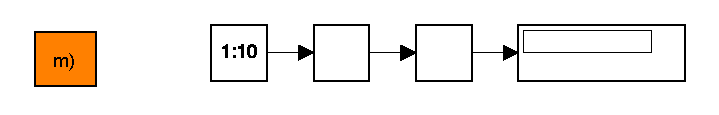
\includegraphics{2m.pdf}}
  \end{figure}
  hvor du ser at i {\sf  Constant}-blokken er 
   tallene for $n$ som \dbox{\sf 1:10} angitt.
   Bruk ellers en {\sf  Math Function}-blokk (velg operasjon fra
   menyen),  en {\sf  Sum of  elements}-blokk og en {\sf 
     Display}-blokk.

   {\color{red}La simuleringstiden fortsatt være  25 sekund.}
Ta med skjermdump av modellen og resultatet.
   
